
We used a laboratory experiment to test if preferences for information are reference dependent. We include a detailed description of procedures and participants in Appendix \ref{appendix:participants}, and the complete survey and instructions to replicate the experiment in the online supplementary material.

\subsection{Experimental design}

\begin{figure}[ht]
  \caption{Structure of the experiment}\label{fig:expDesign}
  \begin{center}
  {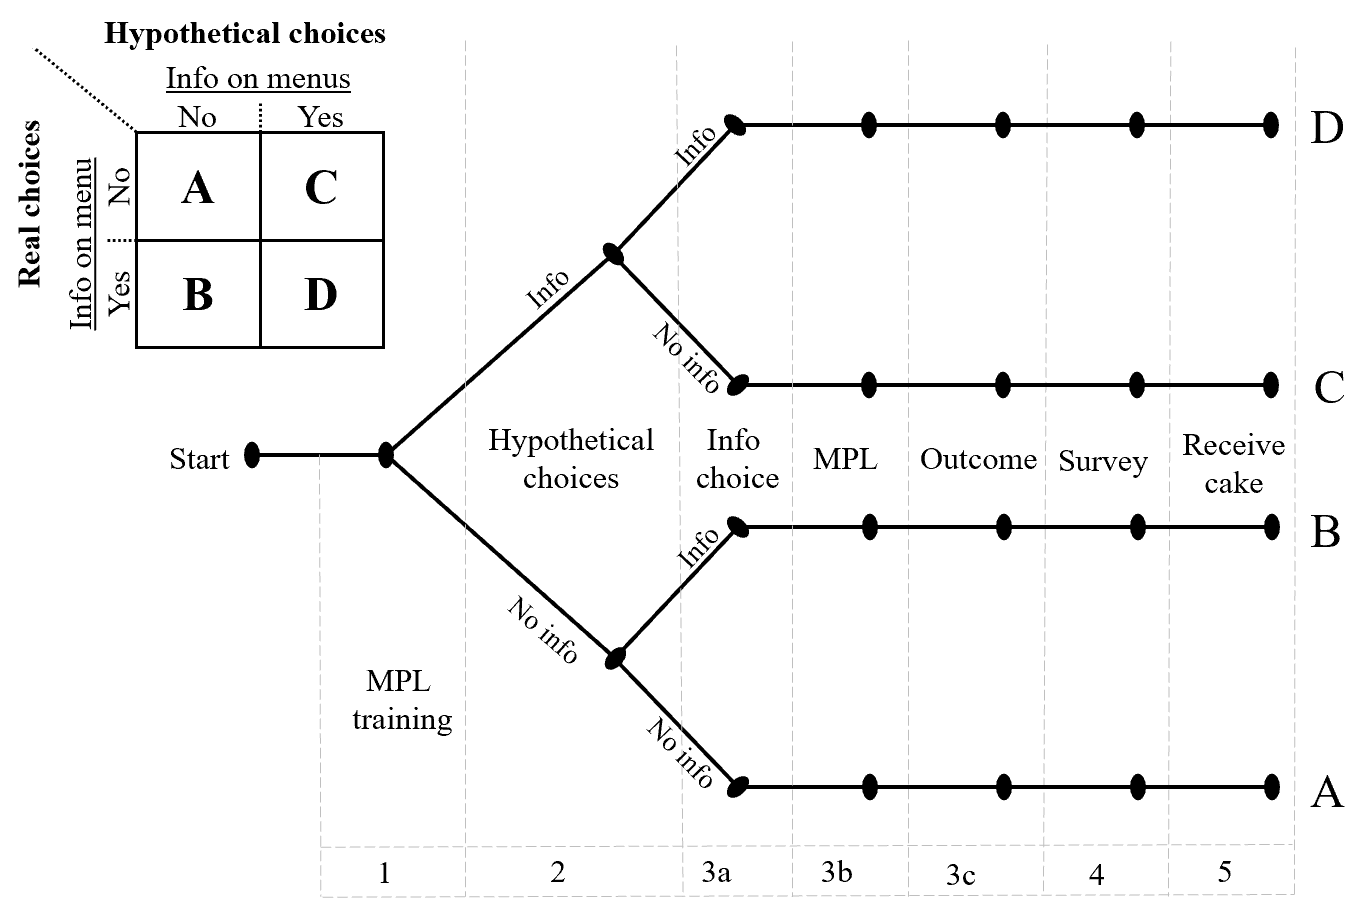
\includegraphics[width=1\textwidth]{./figures/experimentalDesign.png}}
  \end{center}
\end{figure}

Based on our recruitment flyer, all participants knew they would receive a cake for their participation in the experiment. After that, the experiment followed the structure shown in Figure \ref{fig:expDesign}. In step (1), we taught participants how to use a multiple-price list and evaluated their understanding. In step (2), we asked participants to choose their preferred dessert from eleven consecutive dessert menus, each showing three desserts. These choices were not incentivized, and we were explicit about their hypothetical nature. In this step, we randomized half of the participants to see menus without calorie information and the other half to see menus with calorie information. The goal of this manipulation was to exercise some control over potential heterogeneity in expectations about information that participants might have brought to the laboratory. Making a series of choices from menus without (with) calorie information should set a baseline of low (high) expectations of receiving information when moving to the experiment’s next step.

% I DO NOT LIKE THE PARENTHESIS USE ABOVE (!!!!!!!!!!!!!!!!!!!)

In step (3a) participants were once again shown a menu with three desserts. One of these, a cake, was marked as the dessert they were about to actually receive, to eat after the experiment. Within each baseline group established in step (2), we again randomized participants into two groups, resulting in a $2 \times 2$ design. One group was \emph{endowed} with calorie information about the desserts, in the sense that the menu already showed a calorie-information column. The actual calorie numbers were \enquote{temporarily} \emph{xxx}-ed out, however, and participants in this group were asked whether they wanted to \enquote{keep} the calorie information, so they would see it, or \enquote{remove} the calorie information. The exact wording used is shown in Figure \ref{fig:expManipulation} (top panel). The other group was \emph{not endowed} with calorie information, in the sense that the menu showed nothing calorie-related to begin with. Participants in this group were asked whether they wanted to \enquote{add} calorie information, so they would see it, or \enquote{keep} calorie information \enquote{off}. The exact wording used is shown in Figure  \ref{fig:expManipulation} (bottom panel).

\begin{figure}[ht]
  \caption{Key experimental manipulation}\label{fig:expManipulation}
  \begin{center}
  {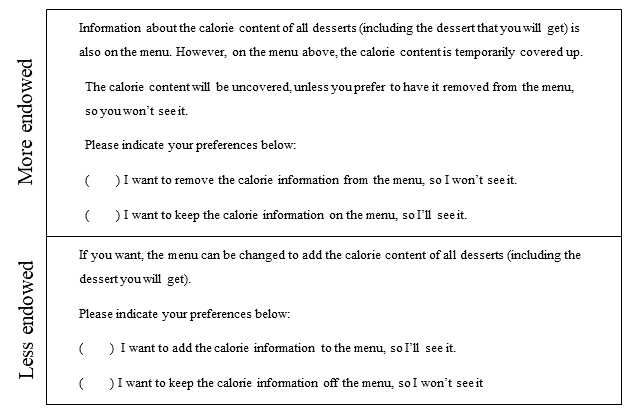
\includegraphics[width=1\textwidth]{./figures/keyManipulation.png}}
  \end{center}
\end{figure}

We argue that, compared to participants in the \emph{not endowed} treatment, participants in the \emph{endowed} treatment were more likely to expect to receive calorie information about their cake, for three reasons. First, the presence of \emph{xxx}-ed out calorie-information column on the menu was intended to make endowed participants focus first on getting calorie information when considering whether they want to actually see it, whereas the absence of any such information for non-endowed participants was intended to make them focus first on not getting it. Second, the menu description pointed to the calorie information as already being on the menu for endowed participants, but as needing a change in the menu for non-endowed participants. And third, the description of how participants could choose to see the information used \enquote{I want to keep} for endowed participants, but \enquote{I want to add} for non-endowed participants.

% check usage of MPL

In step (3b) we aimed to elicit a monetary value for calorie information, using a multiple-price list that allowed this value to range from negative to positive. For example, if participants chose to see the calorie information in step (3a), thereby indicating that information had positive value for them, we gave them the option to either keep the information on the menu (i.e., stick with their initial choice and ultimately see the information) or remove the information and receive some additional money. That is, we elicited their Willingness To Accept (WTA) to \emph{not} see the information after all. Conversely, if participants chose not to see the information in step (3a), thereby indicating that information had negative value for them, we elicited their WTA to \emph{see} the information after all, in a similar fashion.

The multiple-price list included 10 choices, with monetary amounts ranging from \$0.01 to \$5.00.\footnote{The complete list of values in the MPL is \$0.01, \$0.25, \$0.50, \$0.75, \$1.00, \$1.50, \$2.00, \$2.50, \$3.00, and \$5.00.}  Once all 10 choices were made, one choice was randomly selected to be binding.

In step (3c), participants were shown a menu on which the calorie information of the cake they were about to receive was either revealed or not, depending on the outcome of the multiple-price list. In step (4), participants answered survey questions about their demographics, attitudes (risk preferences, time preferences, and degree of self-control), health status, health concern (the importance they assigned to their own health), and familiarity with calorie information (see Appendix \ref{appendix:background} for a description of these data). Finally, in step (5), participants received their payment and cake.

\subsection{Identification strategy}

Based on our two consecutive manipulations to influence participants’ expectations about receiving calorie information, we organize participants in four groups: A, B, C, and D (see Figure \ref{fig:expDesign}). In the first manipulation, participants in groups A and B chose desserts from menus without calorie information, whereas participants in groups C and D chose desserts from menus with calorie information. In the second manipulation, participants in groups A and C chose whether to add information to a menu, whereas participants in groups B and D chose whether to keep information on a menu.

Because we are manipulating expectations, the timing and order of the manipulations matter. Specifically, for participants induced by the first manipulation to have high baseline expectations of receiving information (groups C and D), we expect the effect size of the second manipulation to be smaller. We therefore analyze that effect size separately for each baseline (i.e., groups A and B separately from groups C and D).

For each baseline, we identify the endowment effect by relating our experimental design to our theoretical definition of an endowment effect in equation \ref{eq:endowmentEffect}: $U(L^i|R^i)-U(L^u|R^i)>U(L^i|R^u)-U(L^u|R^u)$. For example, for participants induced by the first manipulation to have low baseline expectations of receiving information (groups A and B), being endowed with information in the second manipulation corresponds to having reference lottery $R^i$ (group B, left-hand side of the equation), while not being endowed corresponds to having reference lottery $R^u$ (group A, right-hand side of the equation). Within each group, choosing to receive information corresponds to choosing outcome lottery $L^i$, while choosing not to receive information corresponds to choosing outcome lottery $R^u$. Thus, we can infer whether $U(L^i|R^i)-U(L^u|R^i)$ is positive ($L^i$ is chosen) or negative for each participant in group B, and similarly infer whether $U(L^i|R^u)-U(L^u|R^u)$ is positive or negative for each participant in group A. Then, we aggregate the choices of each group and simply compare the share of participants in group A who chose to receive information to the share of participants in group B who did so.\footnote{However, we note that our experimental results are contingent on the unverified manipulation of expectations (i.e., probabilistic beliefs). First, we assume that making eleven choices using menus with or without calorie information changes the probabilistic belief to expect to receive information. Second, given the probabilistic belief previously assumed to have been manipulated, we assume that presenting a menu with or without covered calorie information, along with other framing differences, would further change the probability belief to expect to receive information or not. We chose not to verify that the manipulations in fact had the intended effect in forming the expectation to receive information. One alternative would have been to ask participants whether they were expecting to receive information after each manipulation, however, we thought that such verification would have unintendedly changed the expectations. A second alternative would have been to use a different experimental design to manipulate the expectations. Following \citet{marzilliericsonExpectationsEndowmentsEvidence2011} \citet{heffetzEndowmentEffectExpectations2014}, one could manipulate the expectations, for example to expect to receive information, by telling participants that they have a 1\% chance to be able to choose whether to get the information or not, and a 99\% chance to receive the information (more recently, \citet{cerulli-harmsRandomizingEndowmentsExperimental2019} show that forced exchange is preferred than the allowable exchange used by \citet{marzilliericsonExpectationsEndowmentsEvidence2011} and \citet{heffetzEndowmentEffectExpectations2014}). The advantage of this approach is that one can verify that participants formed the correct expectations with a quiz evaluating the understanding of the statement. However, we think that our approach is more appropriate for the context of information and closer to potential policy applications outside of the laboratory. Overall, as reflected by the sensitivity of results to changes in the experimental environment documented in the empirical literature of expectations-based reference-dependent models, we can only conclude that manipulating expectations is a challenging task in which trade-offs are inevitable.} Furthermore, the heterogeneity in the data can be rationalized by assuming random utility.\footnote{Explicitly, participants could be heterogeneous (for example) in terms of self-control, curiosity, or concern about calorie intake.}

Our main goal is to show that preferences for information are not standard, and to propose that these preferences are reference-dependent. Therefore, we use the model of standard preferences as a straw man to set up null hypotheses to be rejected \citet{dellavignaChapterStructuralBehavioral2018}. Explicitly, we test the null hypothesis that the share of participants who choose to receive information is the same regardless of endowment status against the alternative that the share is higher for endowed participants. Note that the distinction between the DA approach and the KR approach does not play any role in the experiment: our design does not set out to distinguish between the two.\footnote{\citet{sprengerEndowmentEffectRisk2015} tests for the existence of an endowment effect for monetary risk using a design that does purposely distinguish between the DA and the KR approach. He shows that the data supports the KR approach instead of the DA approach.}
